% IN THIS SECTION SHOW SOME OF OUR TRANSLATED CODE... AND WALK THROUGH IT THE SAME WAY YOU DID WITH THE CONCEPT IN RESOLVE. BUT BEFORE YOU DO THAT, SHOW THE PICTURE (The one thats already here showing high level relationships and update it!).
\section{Implementation}
Development of our C translation tool can be logically partitioned into three distinct phases: 
\begin{enumerate}
\item Arriving at a translation model (or, strategy) for an accurate C representation of RESOLVE.
\item Implementing reusable mechanisms for carrying out the C code generation process.
\item Creation of a memory manager capable of safely allocating and freeing dynamic memory required by the generated code.
\end{enumerate}
We illustrate each of these phases working in tandem on the LED component discussed in Section \ref{sec:specifiying}. 

\subsection{C Translation Model}
One of the primary challenges in translating from RESOLVE to C is finding a suitable C analog for each RESOLVE module and the constructs allowable in each. Indeed, since we are dealing with an environment where functional correctness is a primary concern, it is important that the code generated by our tool represents as closely as possible the original RESOLVE source. In an effort to make such considerations, at the highest level, the C code we generate makes special considerations for facilities, concepts, and realizations. This scheme is depicted in Figure \ref{fig:relationship} and briefly summarized in Sections \ref{sec:conceptoverview} - \ref{sec:facilitiesrealizations}.

\begin{figure}
\begin{center}
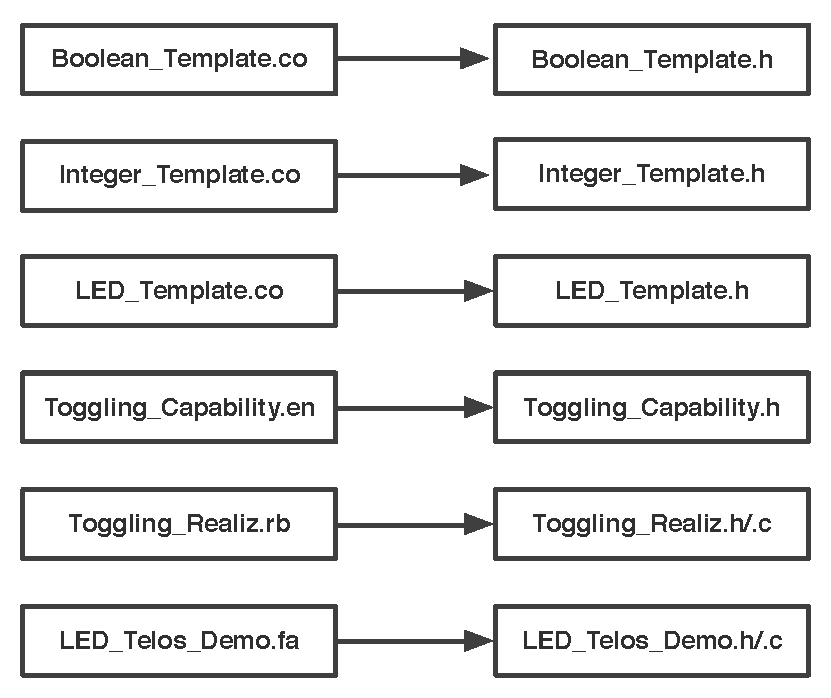
\includegraphics[scale=.60]{figs/relationship.pdf}
\end{center}
\caption{Relationship between RESOLVE module types and the C code generated from each.}
\label{fig:relationship}
\end{figure}

\subsubsection{Concepts}
\label{sec:conceptoverview}
Concept modules produce a single .h file, which provides function pointers for the operations specified in the original concept, as well as structs representing each user defined type. 

\subsubsection{Facilities}
\label{sec:facilitiesoverview}
Facilities produce an .h/.c pair: The header .h declares methods that are intended to manage the creation and destruction of all global variables used within the facility, while the .c provides an implementation of these methods.  Note that these create and destroy methods are only responsible for freeing \textit{global} variables. All other translated local functions are responsible for deallocating their own local variables. 

\subsubsection{Realizations}
\label{sec:facilitiesrealizations}
We treat realizations of concepts and enhancements slightly different than facility modules. While a .h/.c pair is still produced, the create method designated in the header for realizations is designed to create instances of all types specified by the concept, while the destroy method deallocates these types -- as opposed to simply destroying user created globals.

%The memory model must also be considered as an additional verifiable component. Currently, RESOLVE is not capable of creating a complete specification of memory\footnote{RESOLVE is an object based language and has variable sized structures. Using dynamically allocatable memory is the favored approach to allow arbitrarily sized data.}. Thus, a memory model must be realized without a specification. To provide a straight forward translation from RESOLVE to C, we provide a dynamically-based memory allocator for use on embedded systems.

%Unsurprisingly, concepts are represented in C by a single header .h listing the various methods 

\begin{figure*}
\begin{center}
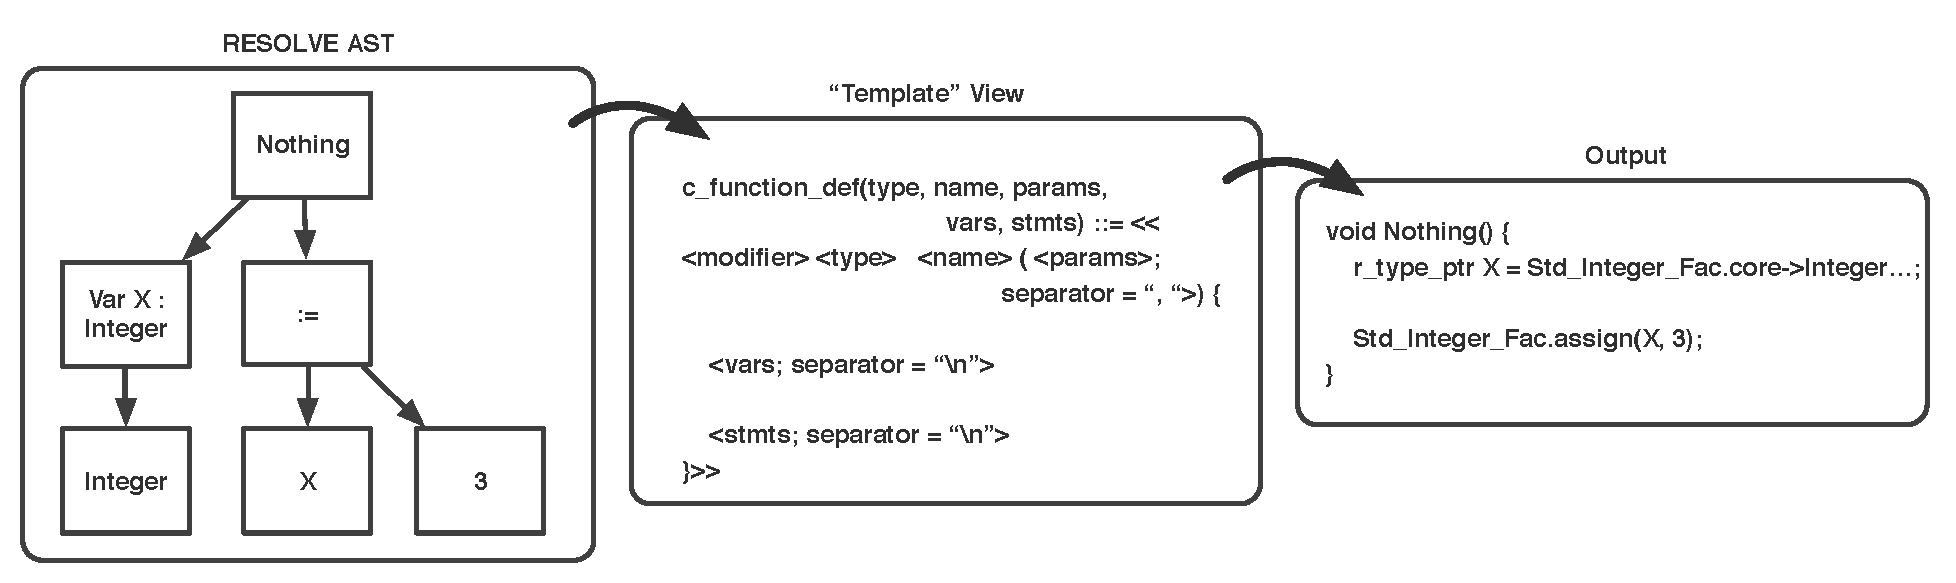
\includegraphics[scale=.55]{figs/ast_traversal2.pdf}
\end{center}
\caption{The general flow of information from C translators walk of the AST (first), to user defined templates (middle), ending with formed output (last).}
\label{fig:ast}
\end{figure*}


\subsection{Translator Implementation}

The C code generation process takes place over the course of a traversal of RESOLVE's abstract syntax tree (AST). The traversal mechanism used is a derivative of the visitor pattern that provides a pre post traversal over all nodes in the tree. 

%\subsubsection{AST Traversal}
%Translation is performed over the course of a traversal of RESOLVE's abstract syntax tree (AST). The traversal mechanism used is a dervivative of the visitor pattern that provides a SAX-dom style pre-post traversal over all nodes in the tree. Thus, for any given node present, a total of two visits occur: One corresponding to the node being `hit' during the pre traversal stage, and one for the post. 

To illustrate the general process of producing runnable C from RESOLVE code, consider the following dummy operation:

\begin{verbatim}
Operation Nothing(); Procedure
        Var X : Integer;
        X := 3;
end Nothing;
\end{verbatim}

%%LOOK AT ME
%This separation between the RESOLVE source tree and the view, allows us to easily modify and tweak the code produced by our tool and allows us easily represent arbitrarily complicated output 

Shown in Figure \ref{fig:ast} is a high level depiction of steps taken in translating this operation to C. The first box depicts the AST of \texttt{Nothing}, where nodes are represented with boxes labeled by the constructs they contain. Throughout the walk of this tree, useful information (such as the operation's name, ``Nothing") are extracted from the nodes containing these constructs, and added to the externally defined string-template\footnote{A template can simply be thought of as a ``document with holes" which the user choses when and how to fill}, \texttt{c\_function\_def} template.

In the context of RESOLVE to C translation, these templates, when filled during the aforementioned pre-post visitor traversal of RESOLVE's AST, help simplify the task of producing complicated, arbitrarily nested blocks of structured C output by keeping translation logic strictly within the C translator, and output logic strictly within the templates.

That is, the only actual work being performed within the C translator is forwarding information gathered from individual treenodes, to a series of externally defined templates. This allows us to exploit (in design pattern parlance) a strict model view controller (MVC) separation in the translator's codebase between the mechanism that does the AST visiting (controller), the tree nodes from which we're adding information to templates (model), and the external file containing all available C language templates which shape our output (view).

We feel this approach lends itself the challenge discussed in this paper, as this separation allows us to easily iterate changes to our generated C code without needing to concern ourselves with a line of Java inside the compiler itself. This allows us to easily tweak code and make arbitrarily complicated changes and optimizations to the code -- some of which are detailed later in Section \#.

% general flow Each of these calls are received in the translator in the order in which they are visited within the tree. It is up to the client (in this case, the author of the C-translator) to decide which of these methods they wish to override and perform custom actions within. 

%\subsubsection{Translation output}
%Output of translated code is done using \textit{Stringtemplate} -- a third-party tool written in Java that allows users to define parameterizable templates. Like the name suggests, a template is simply ``a document with holes" that the user choses when and how to fill. 

%An example C function definition template is shown below.

%\begin{verbatim}
%function_def(modifier, type, name, params, 
%                               vars, stmts) ::= <<
%<modifier> <type> <name> (<params; sep = ", ">) {
%    <vars; sep = "\n">
%    <stmts; sep = "\n">
%}>>
%\end{verbatim}

%User supplied attributes, enclosed in \texttt{<..>}, indicates the position of that attribute relative to others. It is entirely up to the user to define which attributes to fill in, and how complex they want them to be. For example, the user might choose to fill the \texttt{params} attribute with a simple string, or a separately defined \texttt{parameter} template, which in turn might use another separately defined \texttt{type} template.

%\begin{verbatim}
%parameter(type, name) ::= "<type> <name>"
%\end{verbatim}

%In the context of language translation, these templates, when stored on a stack and manipulated over the course of the aforementioned AST traversal, help simplify the task of producing complicated, structured blocks of C output. For instance, upon visiting \texttt{preOperationDec}, a \texttt{function\_def} template can be instantiated by the client and pushed onto a global translation stack with its \texttt{name}, return \texttt{type}, and \texttt{modifier} attributes filled in. As \texttt{preOperationDec}'s children are visited, the \texttt{function\_def} template currently at the top of the stack receives similarly constructed parameter, variable, and statement templates from the nodes being walked. Upon reaching \texttt{postOperationDec}, we can be assured that the function has been completely filled in with the appropriate templates -- assuming the user has implemented the children's visit methods.

%Hence, the only actual work being performed within visit methods is forwarding appropriate information from tree-node it represents, to an externally defined template. This allows us to exploit (in shameless design pattern parlance) a strict model view controller (MVC) separation in the translator's codebase between the mechanism that does the AST visiting (controller), the tree nodes from which we're adding information to templates (model), and the external file containing all available C language templates (view).



\subsection{Memory Allocation}

Dynamic memory allocation is not typically the first choice for most embedded applications. With the telos mote itself  limited to 128 bytes of RAM, hardware and memory constraints such as these, developers of embedded applications tend to favor static memory allocation over dynamic. Many programs, however benefit greatly from dynamic memory allocation not only in terms of clarity and straightforward to be used, including RESOLVE, in order to make it extensible. Previous RESOVE translations to C required static memory allocation \cite{regula:2010}. In this section a stack based dynamic memory allocator is introduced.

\subsubsection{Allocation using \texttt{salloc}}

The \texttt{salloc()} is a first fit memory allocator. Rather than allocating on the heap, \texttt{salloc()} uses the stack. At compilation, the allocator provisions a fixed size of memory. It requires a small section of meta-data called a block which contains information of about the size of memory allocated, neighboring blocks, as well if the block is free or not. A sample representation of the stack shown in figure \ref{fig:stack}, is a typical example of allocated memory on the stack.

\begin{figure}[!htb]
\centering
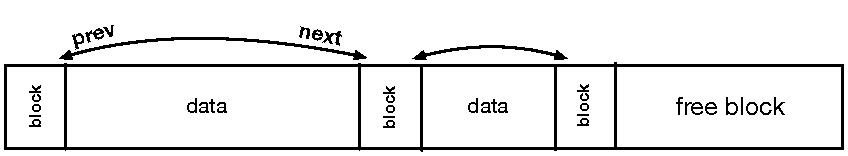
\includegraphics[scale=.55]{figs/stack.pdf}
\caption{Representation of memory stack}
\end{figure}
\label{fig:stack}

\subsubsection{Deallocation using \texttt{sfree}}

A memory allocator must provide a mechanism to release, or free memory in order to indicate that it is not being used and can be reallocated for something else. The \texttt{sfree()} operation is an analogous implementation to the standard C \texttt{free()} function for the stack.

\begin{figure}[!htb]
\centering
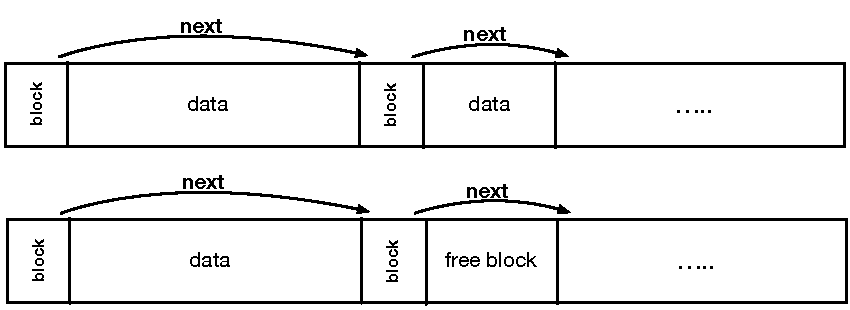
\includegraphics[scale=.55]{figs/sfree.pdf}
\caption{sfree to free memory}
\end{figure}
\label{fig:free}
 
\subsubsection{Optimizations}

A common problem that can occur in memory allocation is fragmentation.  As shown in figure \ref{fig:fragmentation}, fragmentation can lead to inefficient and increased memory usage. This problem is magnified on embedded systems with limited memory capabilities. Simple optimizations can be made however to reduce fragmentation. Splitting is one optimization that \texttt{salloc()} to maximize memory usage. Shown in figure \ref{fig:split}, blocks can be split to the size that is required. Another means of optimizing memory usage is joining together freed blocks. When a call to \texttt{sfree()} is made, neighboring blocks are coalesced together, as shown in figure \ref{fig:fuse}.

\begin{figure}[!htb]
\centering
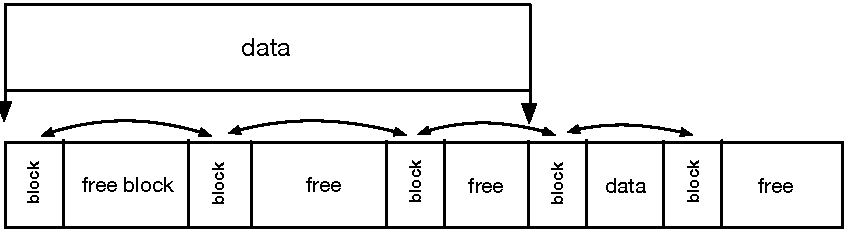
\includegraphics[scale=.55]{figs/fragmentation.pdf}
\caption{fragmentation}
\end{figure}
\label{fig:fragmentation}

\begin{figure}[!htb]
\centering
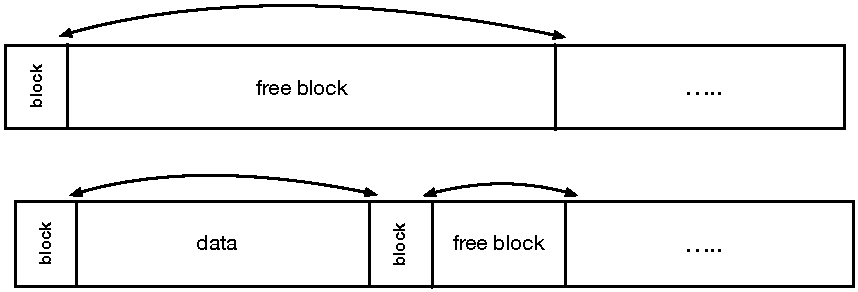
\includegraphics[scale=.55]{figs/split.pdf}
\caption{block splitting}
\end{figure}
\label{fig:split}

\begin{figure}[!htb]
\centering
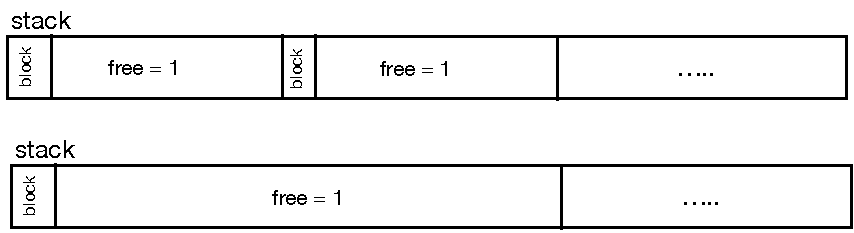
\includegraphics[scale=.55]{figs/fuse.pdf}
\caption{block fusing}
\end{figure}
\label{fig:fuse}
%A stack-based approached to dynamic memory allocation requires a fixed size of memory to be set prior to compilation. 
%To date there have been very few practical applications of verifiable code on physical media. 

\subsection{An LED Implementation}

\begin{verbatim}
void LED_Telos_create() {
		Std_Boolean_Fac_create();
		Std_Integer_Fac_create();
		Std_Clock_Fac_create();
		r_type_ptr __arg_0 = Std_Integer_Fac_Var.core->createFromInteger(4, Std_Integer_Fac_Var.core->Integer);
		LED_Telos_Facility_Var.core = new_Std_LED_Realiz_for_Leds_Template(__arg_0);
		LED_Telos_Facility_Var.Toggling_Capability = new_Toggling_Capability_of_Leds_Template(LED_Telos_Facility_Var.core);
		Std_Integer_Fac_Var.core->Integer->destroy(__arg_0, Std_Integer_Fac_Var.core->Integer);
}
\end{verbatim}